%%%%%%%%%%%%
%%%%%%%%%%%%
\begin{figure}
\centering
%%%%%%%%%%%%%%
\def\xaxis{5}
\def\yaxis{5}
%%%%%%%%%%%%%%
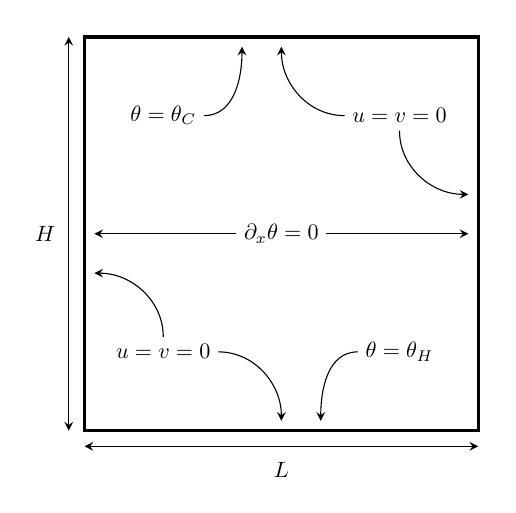
\begin{tikzpicture}[]

	%%% Domain
	\draw[black, very thick] (0,0) rectangle (\xaxis,\yaxis);
	
	%%% Dimensions
	\draw[stealth-stealth] (0,-0.2) -- (\xaxis,-0.2);
	\node[scale=0.8] at (0.5*\xaxis, -0.5) {$L$};
	\draw[stealth-stealth] (-0.2,0) -- (-0.2,\yaxis);
	\node[scale=0.8] at (-0.5,0.5*\yaxis) {$H$};
	
	%%% Velocity BC
	\node[scale=0.8] (bc_top_right) at (\xaxis-1,\yaxis-1) {$u=v=0$};
	\node (bc_top) at (0.5*\xaxis, \yaxis) {};
	\node (bc_right) at (\xaxis, 0.6*\yaxis) {};
	\draw[-stealth] (bc_top_right) to[out=180,in=-90] (bc_top);
	\draw[-stealth] (bc_top_right) to[out=-90,in=180] (bc_right);
	
	\node[scale=0.8] (bc_bot_left) at (1,1) {$u=v=0$};
	\node (bc_bot) at (0.5*\xaxis, 0) {};
	\node (bc_left) at (0, 0.4*\yaxis) {};
	\draw[-stealth] (bc_bot_left) to[out=0,in=90] (bc_bot);
	\draw[-stealth] (bc_bot_left) to[out=90,in=0] (bc_left);
	
	%%% Temperature BC
	\node[scale=0.8] (bc_temp_lat) at (0.5*\xaxis, 0.5*\yaxis) {$\partial_x \theta = 0$};
	\node (bc_left2) at (0, 0.5*\yaxis) {};
	\node (bc_right2) at (\xaxis, 0.5*\yaxis) {};
	\draw[-stealth] (bc_temp_lat) to[out=0,in=180] (bc_right2);
	\draw[-stealth] (bc_temp_lat) to[out=180,in=0] (bc_left2);
	
	\node[scale=0.8] (bc_temp_top) at (0.2*\xaxis, \yaxis-1) {$\theta = \theta_C$};
	\node (bc_top2) at (0.4*\xaxis, \yaxis) {};
	\draw[-stealth] (bc_temp_top) to[out=0,in=-90] (bc_top2);
	
	\node[scale=0.8] (bc_temp_bot) at (0.8*\xaxis, 1) {$\theta = \theta_H$};
	\node (bc_bot2) at (0.6*\xaxis, 0) {};
	\draw[-stealth] (bc_temp_bot) to[out=180,in=90] (bc_bot2);
		
	%%% Redraw domain
	\draw[black, very thick] (0,0) rectangle (\xaxis,\yaxis);
    
\end{tikzpicture}
%%%%%%%%%%%%
\caption{\textbf{Configuration of the sloshing tank.} The fluid flow is determined by the fluid height $h(x,t)$ and by its mass flow rate $q(x,t)$. The movement of the tank is controlled by its acceleration $\ddot{y}(t)$.} 
\label{fig:rayleigh_sketch}
\end{figure} 
%%%%%%%%%%%%
%%%%%%%%%%%%